\documentclass[10pt,a4paper]{article}

\usepackage[hidelinks]{hyperref}
\usepackage{amsmath}
\usepackage[margin=1.5in]{geometry}
\usepackage{graphicx}
\usepackage{caption}
\usepackage{cite}
\usepackage{color}

\begin{document}
\twocolumn
\title{Mobile Robot Systems Mini Project 5}
\author{Sam Sully (sjs252), Paul Durbaba (pd452), Luke Dunsmore (ldd25)}
\date{Lent 2020}
\maketitle
\section{Introduction}
Our project seeks to control a number of robots in a collaborative multi-robot system in order to cover a map in the shortest time. In order to do this the robots will need to localise so that they can report their positions, and thus covered areas. We implement the collaborative localisation strategy presented in Dr Prorok's thesis~\cite{prorok} and compare it with the simpler particle filter implemented in exercise 1 of the Mobile Robots System course.
\section{Localisation}
This section of the project was developed by Sam Sully (sjs252). The approach used was a combination of the sensor-based particle filter used in exercise 1 and the range and bearing approach presented in Dr Prorok's thesis~\cite{prorok}.
\subsection{Particle Filter}
The particle filter works by randomly picking samples (particles) from a proposal distribution and then computing the probability that each particle is correct based on measurements from the robot's sensors. We then re-sample the particles, replacing the less likely ones with more likely ones.

\section{Centralised Navigation}
This section of the project was developed by Luke Dunsmore (ldd25). The focus was on issuing movement instructions to the robots from a centralised server such that the robots cover as much of the world as possible in the shortest amount of time.

\subsection{Partitioning the world}
The benefit of having centralised control is that you can make a fully informed decision about how best to direct the robots. Our approach was to allow the robots to move freely in the world until they were able to somewhat accurately localise themselves. Once they knew where they were, we could assign each robot a portion of the world that it would be their responsibility to cover. We divide the world into regions using the DARP algorithm ~\cite{darp}.

\subsection{DARP}
\label{section:darp}

DARP, which is an acronym for Divide Areas based on initial Robot Positions, takes a world represented as a map of cells, and iteratively assigns the cells to robots. For each robot, there is an evaluation matrix, $E$, which is initially filled with the distance from the robot to each cell in the world. At each iteration after these matrices have been updated, each cell is assigned to a robot as follows:
\begin{equation*}
	A_{x, y} = \underset{i \in {\{1,\hdots,n_r\}}}{\mathrm{argmin}} E_{i|x,y}, \forall(x, y) \in \mathcal{L}
\end{equation*}
where $n_r$ is the number of robots, $E_i$ is the evaluation matrix for the $i$th robot, and $\mathcal{L}$ is the cellular representation of the world. The aim of the algorithm is to divide the world into $n_r$ regions, $L_i$, such that the following conditions hold:
\begin{enumerate}
	\item $L_i \cap L_j = \phi , \forall i, j \in 1, \hdots, n_r, i \neq j$
	\item $L_1\cup L_2 \cup \cdots \cup L_{n_r} = \mathcal{L}$
	\item $|L_1| \approx |L_2| \cdots \approx |L_{n_r}|$
	\item $L_i$ is connected $\forall i \in 1, \hdots, n_r$
	\item $\chi_i(t_0) \in L_i$
\end{enumerate}
where $\chi_i(t_0)$ is the initial location of robot $i$. Each region is determined from the assignments, $A$, as follows:
\begin{equation*}
L_i = \{(x, y) \in \mathcal{L} : A(x, y)=i\}, \forall i \in 1, \hdots, \mathcal{L}
\end{equation*}
Of the conditions listed above, (1) and (2) are taken care of by the fact that the argmin function assigns exactly one robot to each cell. Condition (5) can be handled by allowing a 0 value for cell $(i, j)$ of $E_k$ if and only if robot $k$ is in cell $(i, j)$.

To satisfy condition (3), we iteratively adjust the values in the evaluation matrix. To ensure the regions are of roughly equal sizes, we decrease the values in $E_i$ if $|L_i| < f$, where $f$ is the size of a region obtained through a perfectly equal split of the world, and we increase the values in $E_i$ if $|L_i| > f$.

For condition (4), for each region, $R_i$, that is not continuous we create a matrix, $C_i$, where cells that are close to the section of $R_i$ that the robot is in, and far from the sections that the robot is not in score highly, and cells that are far from the robot's section and close to the other sections score lowly. The evaluation matrix $E_i$ is then multiplied element-wise by $C_i$.

An example assignment of a world to 4 robots is shown in figure~\ref{fig:darp}.

\begin{figure}
	\centering
	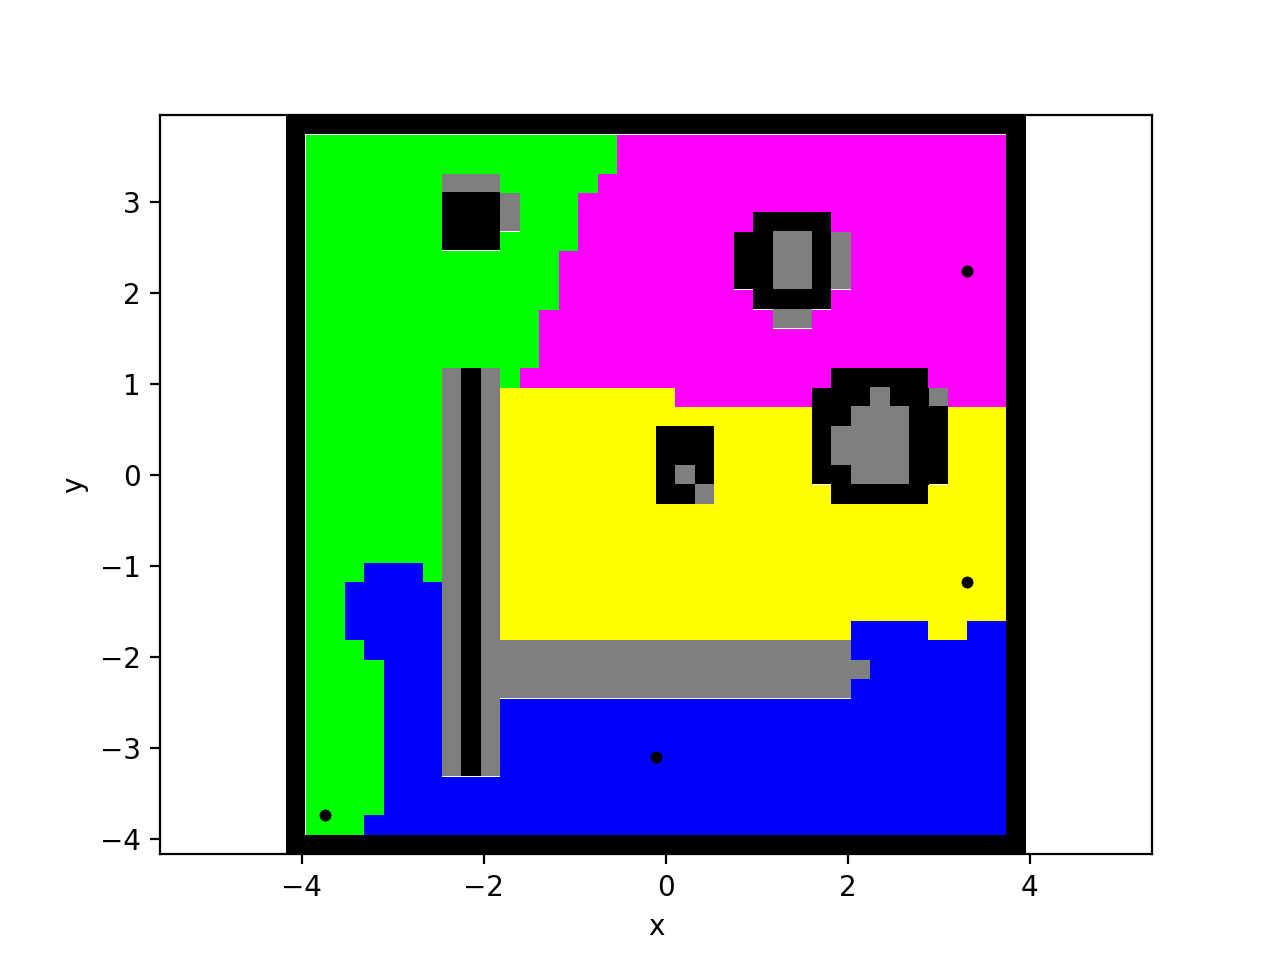
\includegraphics[width=\columnwidth]{figure_darp.png}
	\caption{Division of world into 4 regions.}
	\label{fig:darp}
\end{figure}
   
\subsection{Path Planning}
After each robot is assigned to a region, we calculate a path that it must travel along within its region such that it covers the whole region in the shortest time possible. We aim to do this by minimising the amount of duplicate coverage in the region - that is, covering a part of the region twice, before every part of the region has been covered once. Before running the DARP algorithm, explained in section~\ref{section:darp}, we divide the world into square cells with edges of length double the diameter of the robots. This allows a robot to cover the cell with a single pass in both directions.

After running the DARP algorithm and obtaining a region for each robot to cover, we create a minimum spanning tree that connects the centres of every cell in the region. Since the distance between any two cells are equal, any spanning tree will be a minimum one, so we have freedom to choose edges that will maximise the amount of amount of continuous straight lines in order to minimise time spent turning, which is time not covering new ground. Figure~\ref{fig:mst} shows spanning trees for the three regions.

To generate the final path for the robot, we trace around each of the trees, and we are left with a path that fully covers the region and doesn't cover any section of the region twice.

\color{red}
Somewhere talk about what multi-robot localisation brings to all of this.
\color{black}

\begin{figure}
	\centering
	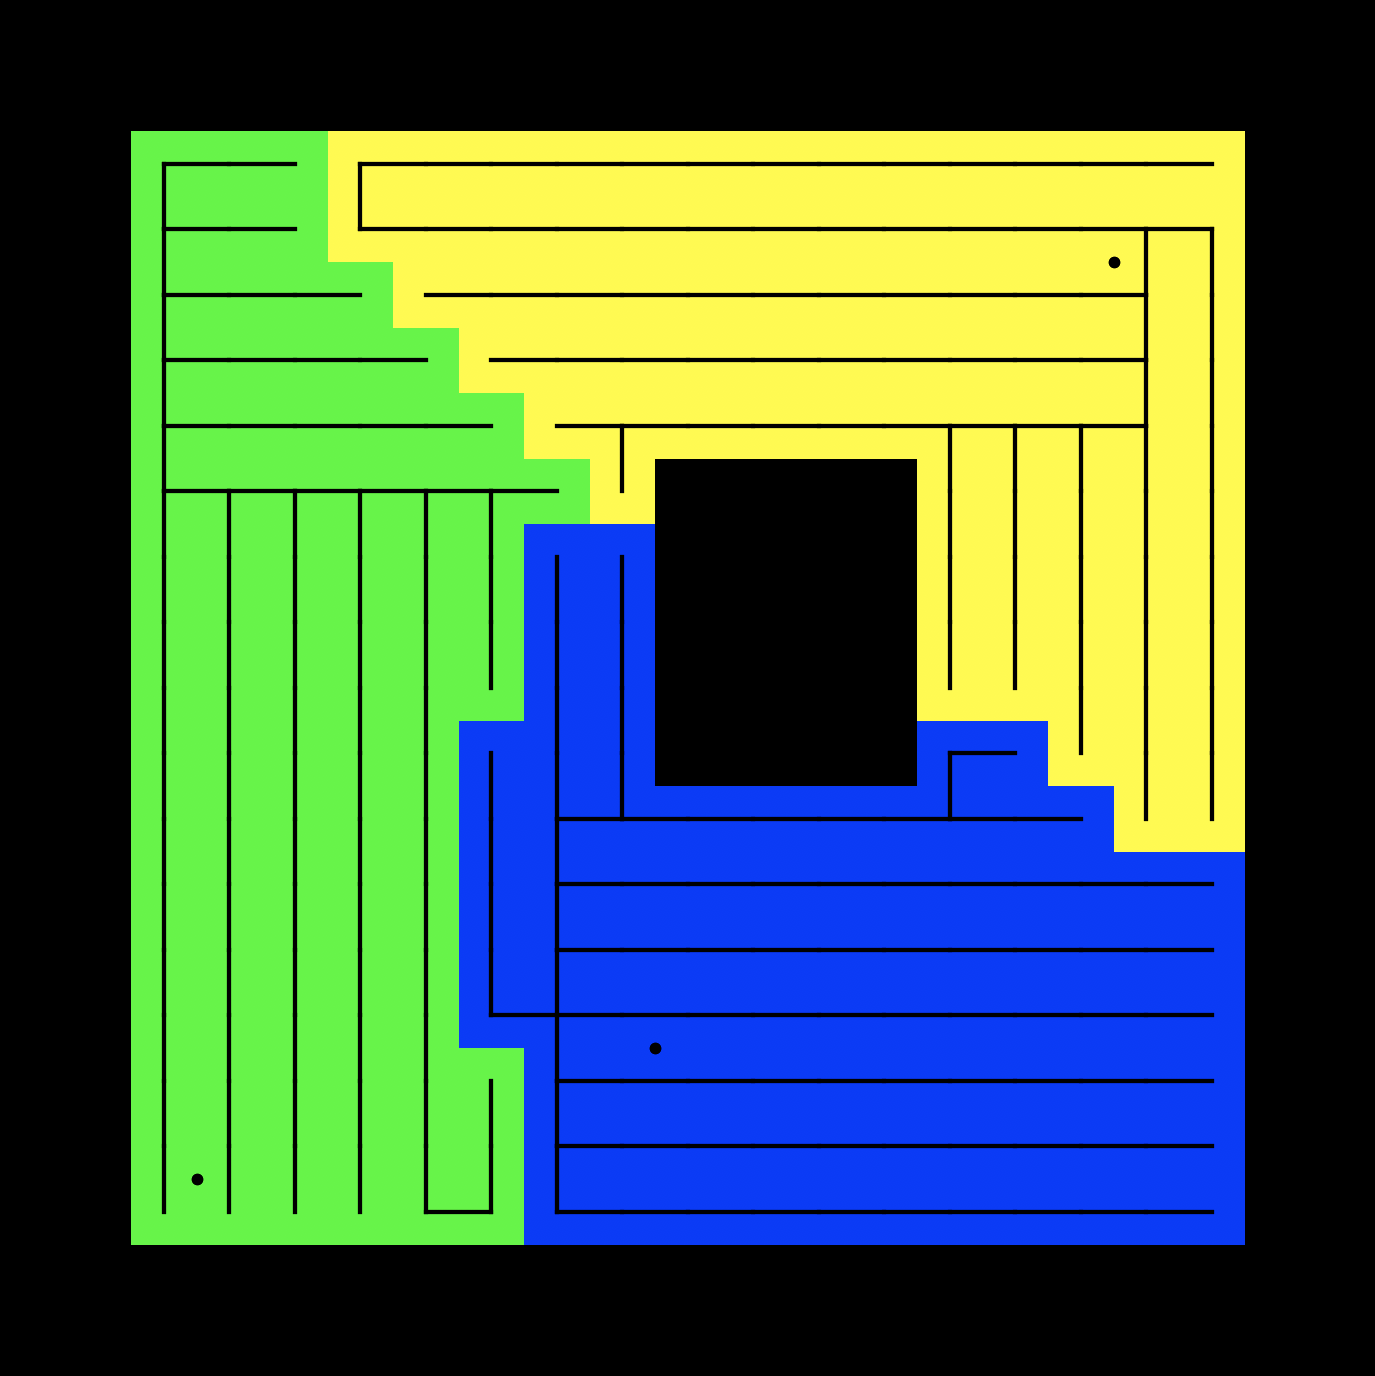
\includegraphics[width=0.8\columnwidth]{figure_mst.png}
	\caption{Spanning trees for each of the three regions.}
	\label{fig:mst}
\end{figure}

\color{red}
\subsection{Path Following}
The final stage of this section was to give movement instructions to the robots so that they 

WRITE THIS SECTION BASED ON THE RESULTS FROM THE EVALUATION
\color{black}

\subsection{Results}
To establish how well this navigation algorithm performs, particularly when it works off predictions of the robots' locations obtained through the localisation algorithm, we first obtained a base performance where we assumed perfect localisation by using ground truth values. We wanted the robots to move as fast as they safely could, so that they would cover the world in the shortest time possible, whilst avoiding collisions and staying on their designated path.

Figure~\ref{fig:ground_truth} shows the rate at which a system using ground truths covered the map, and figure~\ref{fig:ground_truth_coverage} shows the paths that the robots took. We see that the robots had fairly equally sized regions, and completed covering their respective regions at roughly the same time.

\begin{figure}
	\centering
	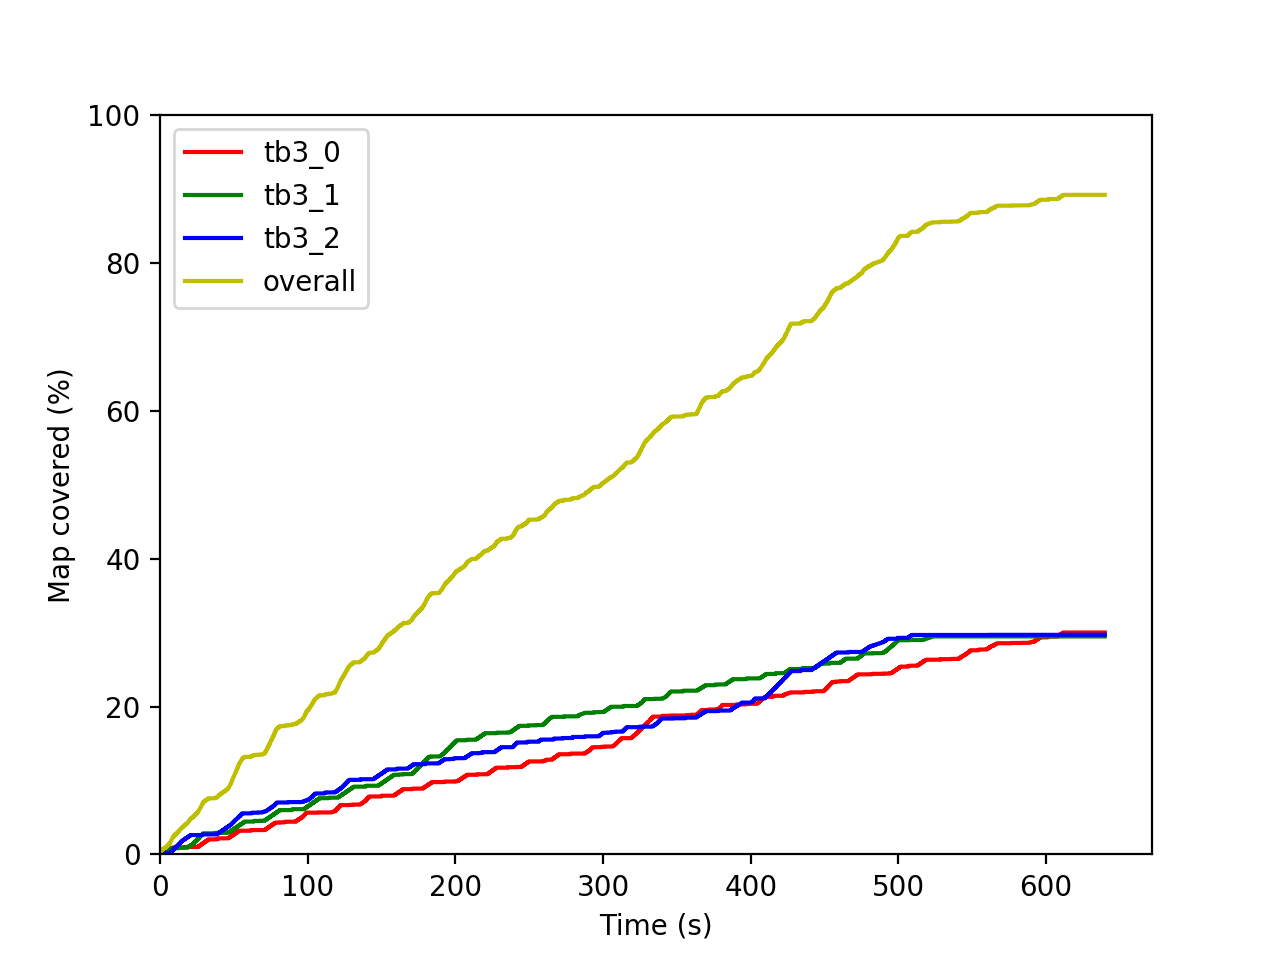
\includegraphics[width=\columnwidth]{ground_truth.png}
	\caption{Progression of world coverage with time.}
	\label{fig:ground_truth}
\end{figure}

\begin{figure}
	\centering
	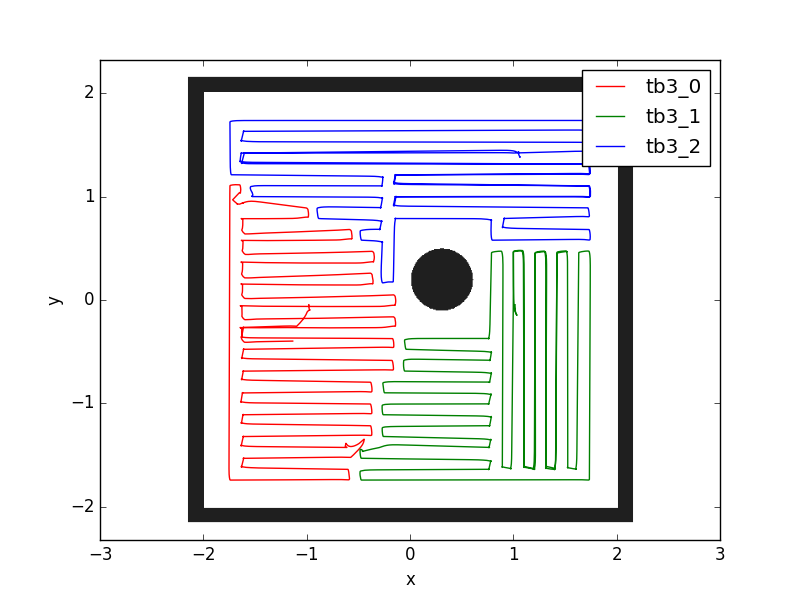
\includegraphics[width=\columnwidth]{ground_truth_coverage.png}
	\caption{Robots' paths to cover the world.}
	\label{fig:ground_truth_coverage}
\end{figure}

SINGLE VS MULTI








\section{Decentralised Navigation}
\section{Evaluation}
\section{Conclusions}
\begin{thebibliography}{9}
\bibitem{prorok} A. Prorok, Models and Algorithms for Ultra-Wideband Localization in Single- and Multi-Robot Systems. 2013.
\end{thebibliography}

\bibliography{mybib}
\bibliographystyle{plain}

\end{document}